\documentclass[10pt,letterpaper]{article}
\usepackage[margin=0.8in]{geometry}
\usepackage[T1]{fontenc}
\usepackage{lmodern,microtype,xurl,booktabs,tabularx}
\usepackage{tikz}
\usetikzlibrary{arrows.meta,positioning}
\usepackage[colorlinks=true,urlcolor=blue,linkcolor=blue]{hyperref}
\setlength{\parindent}{0pt}
\setlength{\parskip}{0.5em}
\newcommand{\source}[1]{\par{\footnotesize Source: \nolinkurl{#1}}\par}
\title{How a Planning Request Moves Through the Software}
\author{Obstacle-avoidance planner}
\date{Source review: 6 September 2026}
\begin{document}
\maketitle

This walkthrough describes the maintained interfaces and execution order.
The numerical examples in \texttt{planner\_manual.tex} are recorded illustrations,
not fresh measurements. Current run evidence belongs in \texttt{benchmark.csv}
and \texttt{verification.md}. The engine's mathematical formulation is maintained
in \texttt{bmtp\_engine\_design.tex} at the repository root.

\section{The public request}

Call \texttt{obstacleAvoidance.planTrajectory} with obstacles, initial state,
goal state, limits, and optional overrides, in that order. A zero-input call
returns independent defaults. Partial and empty overrides retain default values;
unknown fields are ignored with one aggregate warning.

Positions are two-coordinate x/y rows in coordinate units. Times are
seconds. Velocity, acceleration, and jerk limits carry their units in their
field names. Obstacle constructors apply safety margins once and preserve both
original and protected geometry.
\source{+obstacleAvoidance/planTrajectory.m; +obstacleAvoidance/+input/resolvePlannerOptions.m; +obstacleAvoidance/+input/normalizePlannerRequest.m}

\section{The execution order}

\begin{center}
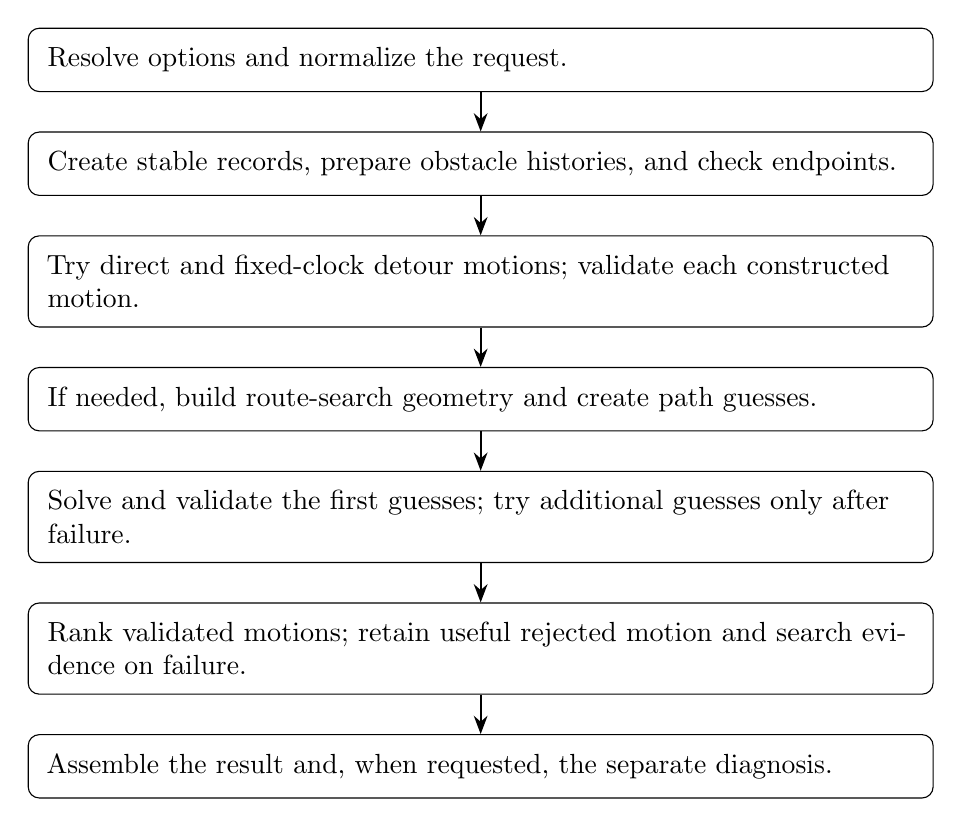
\begin{tikzpicture}[
  stage/.style={draw,rounded corners,text width=11cm,align=left,inner sep=7pt},
  flow/.style={-{Stealth},thick},
  node distance=5mm]
\node[stage] (request) {Resolve options and normalize the request.};
\node[stage,below=of request] (scene) {Create stable records, prepare obstacle histories, and check endpoints.};
\node[stage,below=of scene] (direct) {Try direct and fixed-clock detour motions; validate each constructed motion.};
\node[stage,below=of direct] (routes) {If needed, build route-search geometry and create path guesses.};
\node[stage,below=of routes] (solve) {Solve and validate the first guesses; try additional guesses only after failure.};
\node[stage,below=of solve] (select) {Rank validated motions; retain useful rejected motion and search evidence on failure.};
\node[stage,below=of select] (return) {Assemble the result and, when requested, the separate diagnosis.};
\foreach \a/\b in {request/scene,scene/direct,direct/routes,routes/solve,solve/select,select/return}
  \draw[flow] (\a.south)--(\b.north);
\end{tikzpicture}
\end{center}

Invalid public inputs raise identified errors. An infeasible endpoint returns a
stable expected-failure result. A validated direct motion can return immediately.
A validated fixed-clock detour returns immediately for earliest arrival; fixed
arrival continues to compare travel length with other candidates.
\source{+obstacleAvoidance/+planner/createPlanningRecord.m; +obstacleAvoidance/+obstacles/preparePlanningScene.m; +obstacleAvoidance/+input/validatePlannerEndpoints.m; +obstacleAvoidance/+planner/tryDirectAndFixedTimeMotions.m}

\section{Routes and motion construction}

A path guess supplies geometry or a proposed schedule; it is not a certified
motion. The planner initially considers at most two ordinary guesses.
\texttt{MaximumSeedCount} controls the total ordinary-guess budget; larger
budgets permit failure recovery, which stops at its first validated motion.

BMTP is the obstacle-planning engine. There is no trajectory-method selector.
Static scenes use prepared convex regions. Moving scenes can use a conservative
stationary enclosure, timed-cell BMTP, or a direct wait-and-move construction,
according to the guess's geometry and schedule. Every acceptance still checks
the original protected obstacle histories.

The explicit \texttt{ruckigStopAtWaypoints} fallback is disabled by default.
When enabled, it applies only to supported failure conditions and at most two
route segments. Its forced interior rest states and outcome remain visible.
\source{+obstacleAvoidance/+search/createPathGuesses.m; +obstacleAvoidance/+search/searchRoutes.m; +obstacleAvoidance/+planner/solvePathGuess.m; +obstacleAvoidance/+planner/solveDynamicPathGuess.m; +obstacleAvoidance/+planner/tryAdditionalPathGuesses.m}

\section{The BMTP boundary}

The obstacle adapter supplies numeric exclusion regions to a dimension-neutral
engine. Degree-eight Bezier trajectory calculations and separating-plane
calculations use MATLAB \texttt{coneprog}. Sampled overlap screening guides
iteration; it is not a continuous collision certificate. The engine prepares
and certifies its final polynomial motion before the planner's independent check.
Travel refinement preserves the retained arrival policy and all physical limits.
\source{trajectory/+bmtpEngine/solve.m; trajectory/+bmtpEngine/solveAlternatingTrajectory.m; trajectory/+bmtpEngine/refineTravel.m; trajectory/+bmtpEngine/prepareFinalMotion.m; trajectory/+bmtpEngine/checkFinalMotion.m}

\section{Independent validation and returned evidence}

The public validator checks sampled-history consistency, continuous polynomial
bounds, continuity, endpoint states, workspace, obstacle histories, and applicable
velocity, acceleration, and jerk limits. Unresolved collision certification is
not success. Preparation and pure geometry routines may be shared; acceptance
does not trust a solver success flag alone.
\source{+obstacleAvoidance/validateTrajectory.m; +obstacleAvoidance/+validation/validatePreparedTrajectory.m; +obstacleAvoidance/+validation/validatePolynomialTrajectory.m; +obstacleAvoidance/+validation/checkObstacleClearance.m}

Only validated candidates are ranked. Earliest arrival orders by arrival time,
then motion length; fixed arrival orders by motion length. Failure can retain a
constructed rejected motion and its failed validation, while \texttt{Success}
remains false and the selected route is empty.

The first output preserves the motion, request, and validation inputs.
The optional diagnosis preserves attempts, routes, search traces, solver details,
selection evidence, and timing. First-validation time includes an accepted
fixed-clock detour even when later guesses are attempted. Candidate solving time
excludes validation, consistently with the exclusive stage totals.
\source{+obstacleAvoidance/+planner/selectValidatedCandidate.m; +obstacleAvoidance/+planner/assemblePlannerOutputs.m; +obstacleAvoidance/+planner/createCandidateSummary.m}

\section{Limits and verification}

The finite route search and local motion optimizer do not establish completeness
or global optimality. Moving-obstacle feasibility need not be monotone in time.
Failures distinguish unavailable constructions and unsuccessful validation without
claiming physical infeasibility. MATLAB planning is interrupted with Ctrl+C;
there is no cooperative cancellation callback.

For current verification scope, read \texttt{verification.md}. Benchmark comparisons
must check declared scenario outcomes and fresh independent validation as well as
physical equality. Historical measurements and retired implementations remain
labeled as historical evidence.
\end{document}
